\section{GPGPU}
A Graphics Processing Unit (GPU) is traditionally considered to be an integral part of a workstation computer mainly because it enables accelerated or even real-time rendering of three-dimensional computer graphics. As such, the device relies on a highly specialized and massively parallel architecture. Within a single second hundreds of millions of geometric operations (i.e.\ translation, rotation, scaling) and rendering procedures (i.e.\ interpolation, shading) are applied independently to the polygon primitives of a model by the numerous streaming microprocessors the GPU consists of. Due to the application specific design and since almost all parts of the rendering pipeline are hardware-accelerated, i.e.\ functionality is directly implemented in the physical circuit layout, throughput and computing performance of GPUs are orders of magnitude larger than what a common Central Processing Unit (CPU) can achieve for the same computation. Figures \ref{fig:peakperf} and \ref{fig:memorybandw} show the theoretical peak performance and the memory-bandwidth of selected CPU and GPU models over time. 

\begin{figure}
\centering
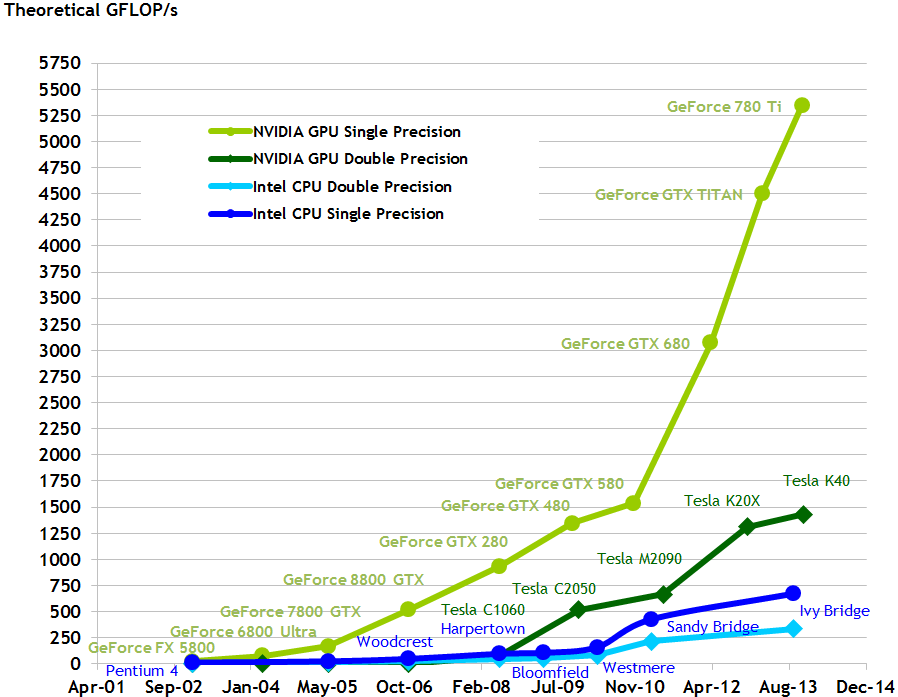
\includegraphics[width=\textwidth, trim = 0mm 0mm 0mm 10mm, clip]{images/floating-point-operations-per-second.png}
\caption{Theoretical peek performance of selected Intel CPU and Nvidia GPU models measured in Giga-Floating-point Operations Per Second (GFLOP/s). Image by Nvidia (cite!)}
\label{fig:peakperf}
\end{figure}

\begin{figure}
\centering
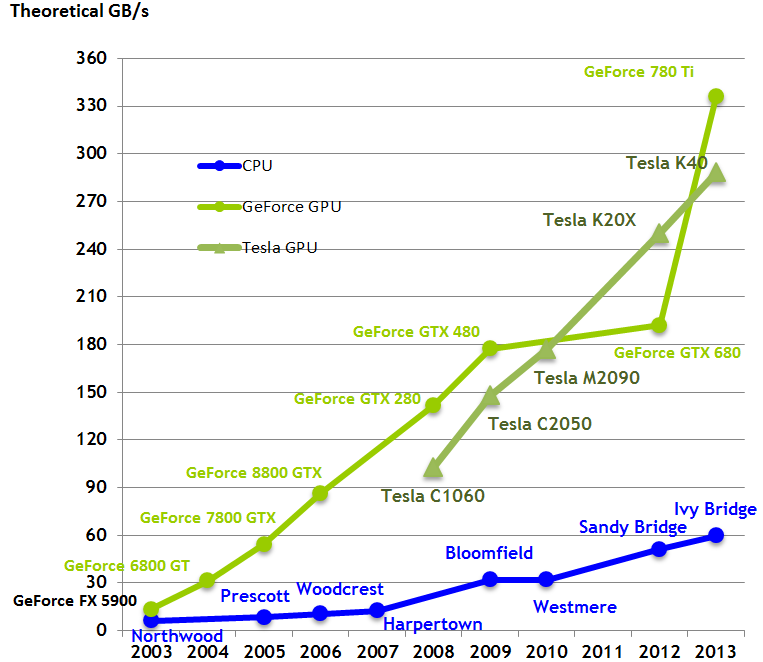
\includegraphics[width=\textwidth, trim = 0mm 0mm 0mm 10mm, clip]{images/memory-bandwidth.png}
\caption{Memory bandwidth of selected Intel CPU and Nvidia GPU architectures measured in Gigabytes Per Second (GB/s). Image by Nvidia (cite!)}
\label{fig:memorybandw}
\end{figure}

In order to benefit from this enormous computational power, research has been conducted to investigate if GPUs can be used to accelerate computations beyond the intended scope \cite{harris_physically-based_2002, owens_gpus_2004}. Since the application programming interface (API) of the devices only supported computer graphics development in these days and due to the fact that a lot of the functionality on the device is hardwired, a general problem has to expressed in terms of pixels, textures and shaders. This process requires a lot of experience, detailed knowledge about the hardware and computer graphics programming as well as trial and error optimization. Apart from these practical hurdles, it turned out that a lot of parallel algorithms, i.e.\ algorithms that consist of independent subproblems that are processed in parallel, can outperform an equivalent CPU implementation by orders of magnitude. 

The term General Purpose Computation on Graphics Processing Unit (GPGPU) was coined by Mark Harris in 2006 \cite{luebke_gpgpu:_2006}. At around the same time, GPU manufacturers realized that scientific computing might be a new market for their products. However, in order to enable the average researcher to harness the computing horsepower of the GPU, improvements in both hardware and software had to be made:
\begin{description}
\item[Hardware] Over the course of subsequent GPU generations, the flexibility as well as the programmability of the streaming multiprocessors (also called shading units or shader) has increased. Furthermore, essential primitives for concurrent programming such as synchronization and atomics were introduced and optimized. In addition, standard CPU features that were formally not available on GPUs like an automatically managed cache or double-precision floating-point arithmetic were added. Both major vendors of GPUs, AMD and Nvidia, have introduced special versions of their devices for professional high performance computing (HPC) applications. Those products, branded AMD FireStream and Nvidia Tesla, respectively, are optimized for use in multi-GPU cluster located in computing centers. 
\item[Software] At an even faster rate than hardware improvements, software innovations were presented. At first, native development in widely-known high-level languages such as C or C++ was enabled\footnote{The language dialect used for GPU development is usually not absolutely compliant with the original standard language. On the one hand some minor language features are sometimes ommited (i.e.\ CUDA-C does not support function pointers), on the other hand small additions are added to account for GPU-specific features and properties.}, later bindings for Python, Java, MATLAB and others were provided. In a next step, highly optimized compilers, debuggers, performance analysis tools and complete integrated development environments (IDE) were shipped to further improve development efficiency and product performance. Furthermore, libraries for applications such as linear algebra (BLAS, SPBLAS), signal processing (FFT) and random number generation were introduced. Now, an existing application can be accelerated just by replacing the library used, without writing a single line of GPU code. 
\end{description}

Over the years, several programming frameworks and standards for GPGPU were introduced. In the following a short overview is given.  
\begin{description}
\item[OpenCL] The Open Computing Language is an open standard for computation on heterogeneous platforms. As such, it can not only be used for GPU programming, but also to create applications that make use of systems that consist of numerous CPUs and so-called accelerators\footnote{Field Programmable Gate Array (FPGA), Digital signal processor (DSP), GPU}. It is based on the C/C++ programming language. The standard has been adapted by over 30 companies, including AMD, Intel and Nvidia. OpenCL 1.0 was introduced in December 2008, the latest version OpenCL 2.0 published in November 2013 includes novel execution models and introduces features of C++11. (cite)
\item[OpenACC] The Open Accelerators standard is developed by several companies including Cray, Nvidia and PGI. OpenACC is conceptually similar to the widely-used Open Multi-Processing (OpenMP) standard for parallel programming in shared memory systems (see chapter ??). The framework primarily consists of a set of compiler directives that can be used to mark regions that are to be run on an accelerator device. The main advantage of this approach is that the developer does not need to know the details of a potentially complicated framework, but can still significantly improve the performance of existing code just by adding compiler directives. Version 2.0a of the standard was ratified in August 2013. 
\item[CUDA] The Compute Unified Device Architecture is a proprietary framework developed by Nvidia. An initial beta version was published in February 2007. Due to its widespread and early distribution on the market and the large number of libraries, tools and resources available, CUDA is considered to be the marking leader for GPU computation. The GPU implementation of the tau-leaping algorithm presented in this thesis is based on CUDA. The most recent version, CUDA 6.0, was published in April 2014. It provides a unified view on CPU and GPU memory and improved scaling for multi-GPU systems. In the following section more detailed information on the paradigms and features of CUDA will be given. 
\end{description}

\ifdebug
\begin{itemize}
\item General-Purpose computation on Graphics Processing Units
\item GPGPU allows the developer to exploit the great computational power of modern GPU by giving access to the underlying parallel architecture that was conceived for speeding up real-time three-dimensional computer-graphics. (Nobile)
\item What is the difference between CPU and GPU
\item Trends
\item What kind of problems are suited for GPU?
\item Modern GPU are throughput-orientated devices with massively parallel architecture. The model used for the simulations ... TFLOPS. 
\item Avoid branches
\end{itemize}
\fi

\subsection{Nvidia CUDA} \label{ch:cuda}
The Nvidia CUDA computing platform combines two major paradigms of modern data processing devices: \textit{Single Instruction, Multiple Data} (SIMD) and \textit{multi-threading}. Following the data parallelism approach, the former principle describes the ability of a processor to apply the same operation to different pieces of data at once. The later, on the other hand, distributes independent instruction streams (\textit{threads}) to the available processors. 

The abstract principles mentioned above can be derived directly from the actual hardware architecture of the device: A Nvidia GPU consists of an array of \textit{Streaming Multiprocessors} (SM) which in turn are formed by a number of so-called \textit{CUDA-cores}. Following the SIMD principle, a SM can only execute one instruction at a time, i.e.\ all cores have to apply the same operation to their current data point. If there is code branching within the instructions issued to one SM, individual cores may skip the operations of a non-applicable branch. This leads to serialization of the execution so that in general branching should be avoided whenever possible. 

Within the instruction stream running on a SM data parallelism is expressed using the SIMD principle. On a larger scale, considering only the multiprocessor units and their in general different instruction streams, task parallelism can be observed. Analogous to the cores within a conventional CPU, all SMs execute at the same time and so do the threads running on them. On Nvidia GPUs, however, communication and synchronization between threads is limited. 

From the point of view of a software developer, a CUDA program consists of code for the host (i.e.\ the CPU) and the device (i.e.\ the GPU). Device procedures, so-called \textit{kernels}, must be launched in the host section of the application. The kernel is then automatically replicated many times to create individual threads. In CUDA, threads are organized in one-, two- or three-dimensional structures called \textit{blocks}, which in turn are part of a \textit{grid}. The size of a block is limited by the hardware and so is the size of blocks and grids. Threads within a block can be synchronized during execution of the kernel, on a global level, however, the only way of synchronizing all threads is the invocation of two destinct kernels. The device assigns blocks to SMs and further splits them to form batches of 32 threads named \textit{warp}. Since the number of threads per warp is equal to the number of cores per SM, a warp can be executed directly. Each thread can determine its position in grid, block and warp at runtime. The complex dispatch and scheduling procedure allows CUDA programs to achieve good performance on different GPUs independent of the properties of the specific model (e.g.\ number of SMs). Figure \ref{fig:cuda_threads} visualizes the concepts introduced above. 

\begin{figure}
\centering
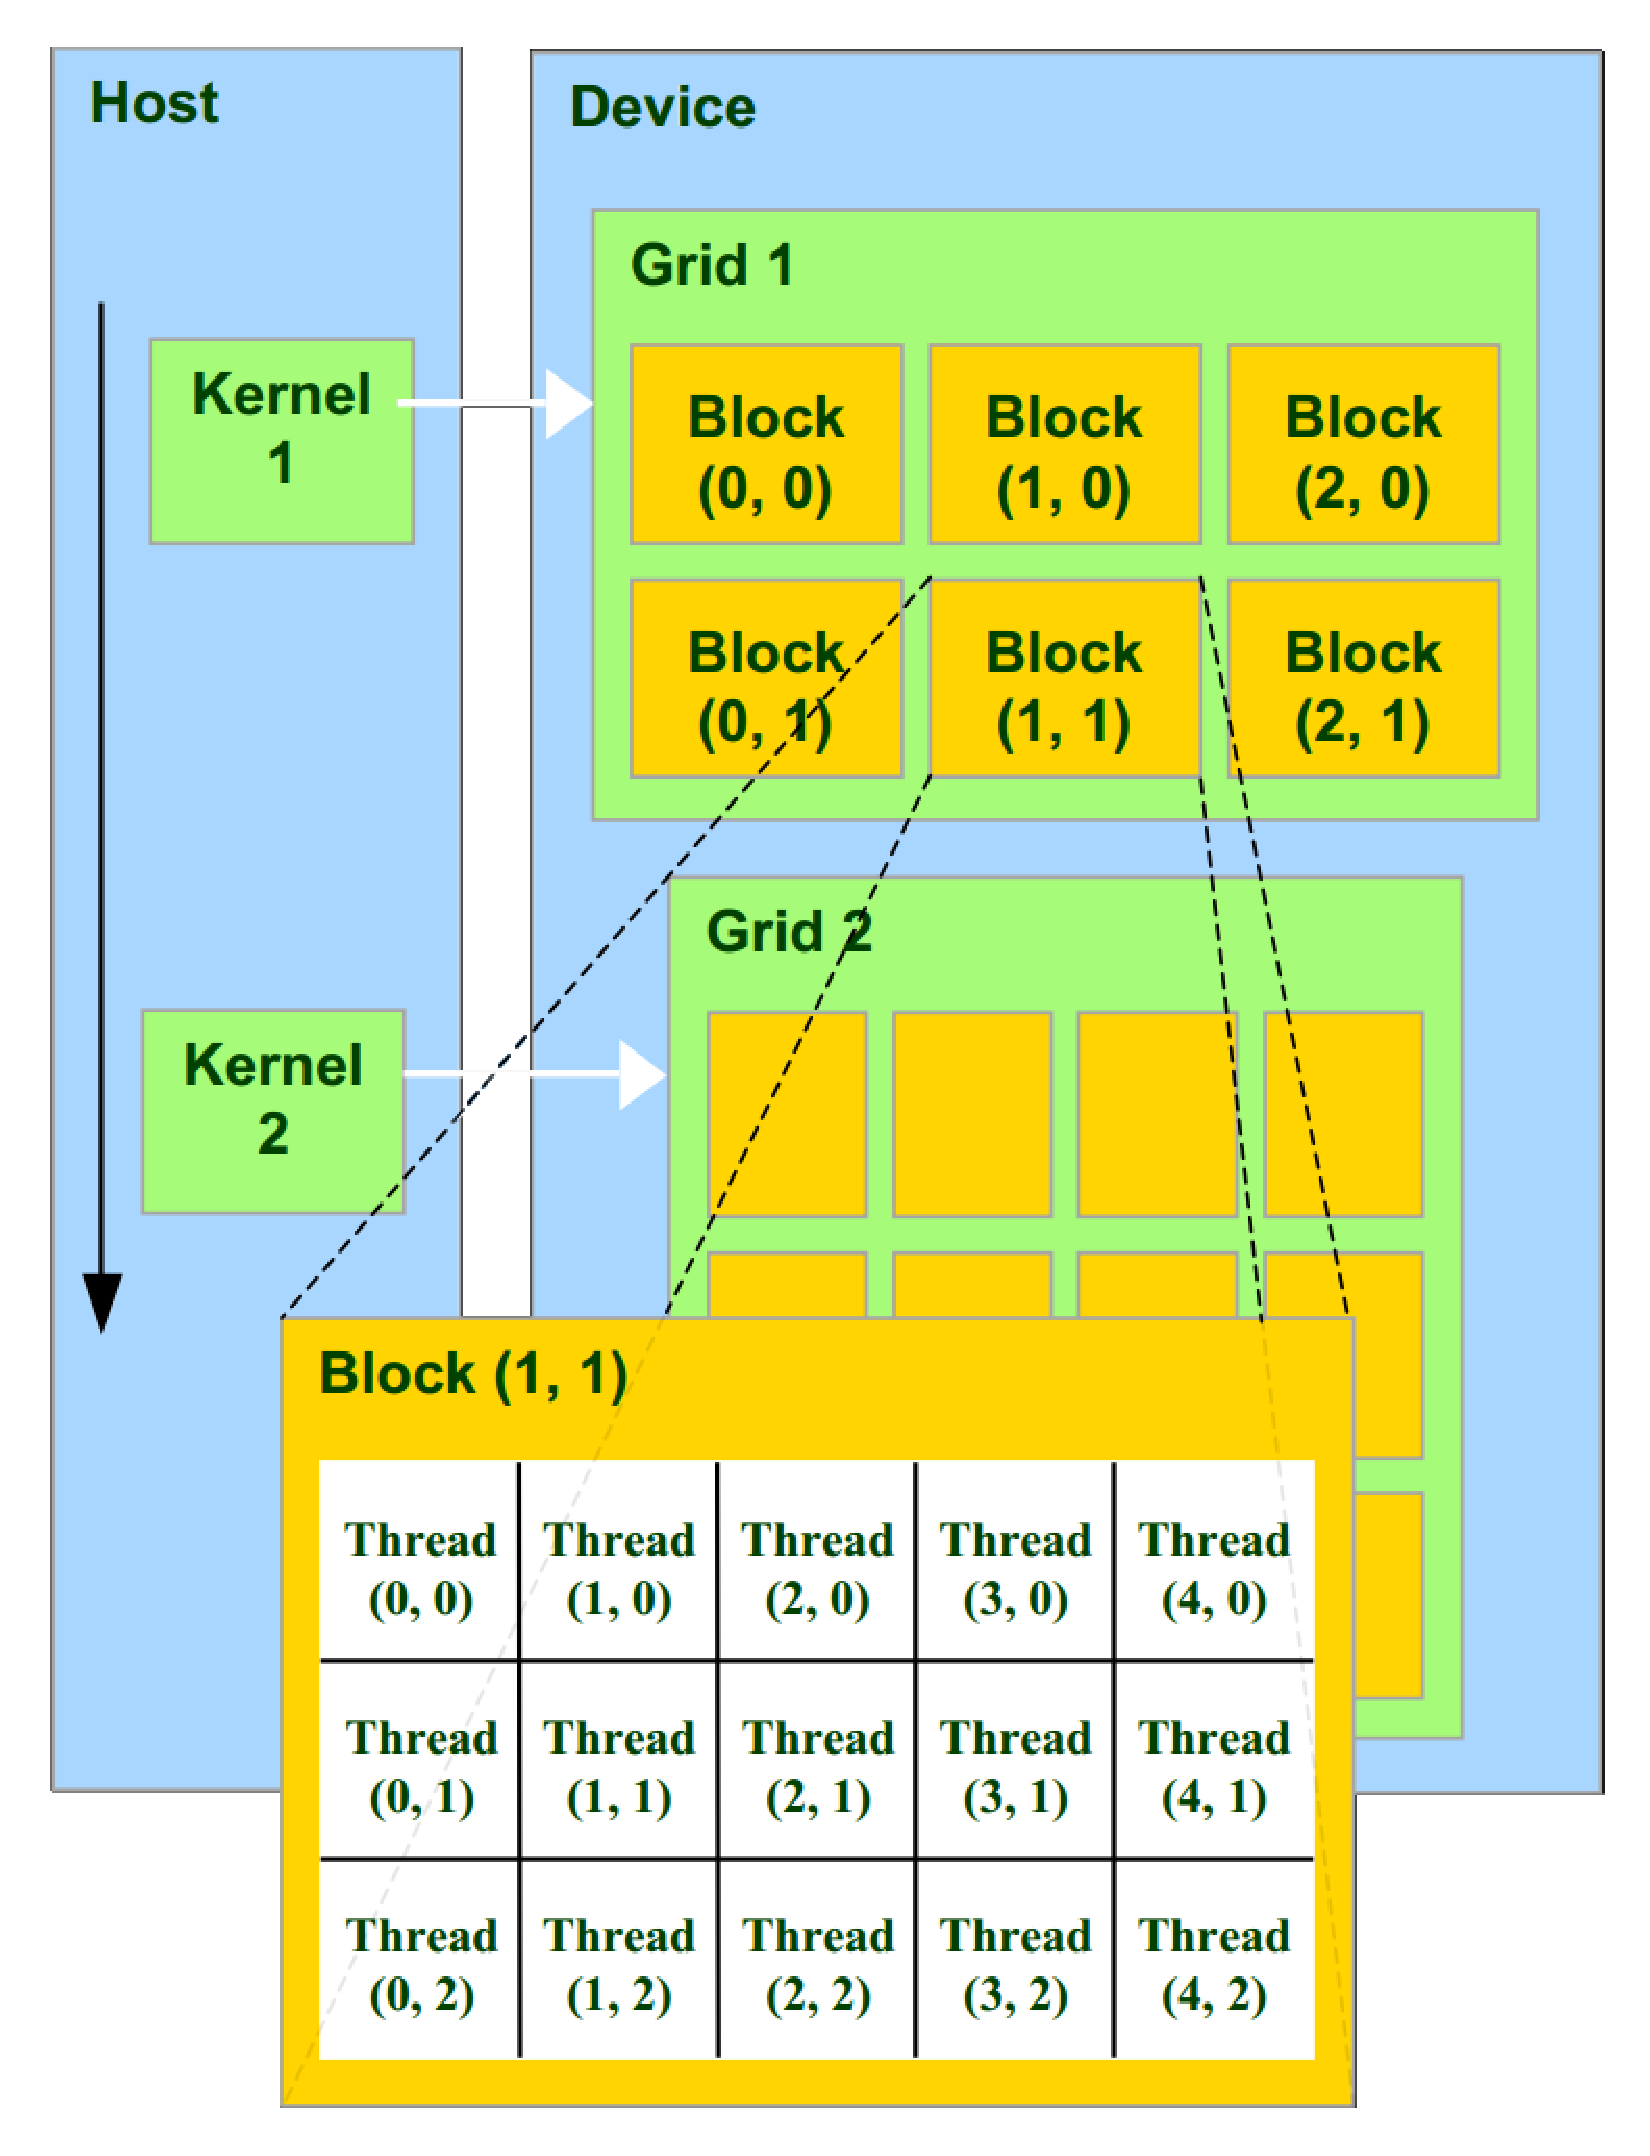
\includegraphics[height=10.0cm]{images/cuda_threads.eps}
\caption{Illustration of the CUDA programming model. Figure taken from \cite{nvidia_cuda_2012}.}
\label{fig:cuda_threads}
\end{figure}

One of the most important aspects to consider when developing GPU applications is the memory hierarchy of the device. Figure \ref{fig:memoryhier} gives an overview over that different kinds of memory on the device, table \ref{tab:bwandaccess} lists bandwidth and latency. 
\begin{description}
\item[Global memory] Global memory can be considered to be the GPU equivalent of the CPU main memory. Its capacity usually exceeds several gigabytes, the bandwidth is in the order of 100 GB/s (see figure \ref{fig:memorybandw}). It is the only kind of memory that can be accessed directly from the host CPU via the PCI-Express port ($\sim$6 GB/s). (some additional sentences)
\item[Shared memory] Data in shared memory is private per thread-block, i.e.\ it can only be accessed by the threads in a block for data exchange. After the complete block has finished execution, its data in shared memory cannot be accessed any more. Physically shared memory is located in banks close to the individual SMs. The bandwidth is usually around 7-10x faster than global memory bandwidth. Since accessing the latter often limits the overall performance of a CUDA application, shared memory can help to reduce the number of expensive global memory transactions by keeping data that is used more than once close to the SM (spatial locality). It is often considered to be a programmer-managed L1 cache. In fact, modern GPUs have an automatically managed L1 cache which physically shares its banks with the latter.  (cite cuda handbook, kaufmann)
\item[Registers] One of the main difference between GPUs and CPUs is the number of registers available. Registers are small but extremely fast memory units that usually only store one single value. They are located very close to the processor such that its content can be fetched almost instantly (i.e.\ within a single clock cycle). A standard multi-core CPU performs best if it can execute a small number of threads in parallel. If the number of threads occupying the processor grows, the overall performance decreases since frequent context switches are needed to ensure that every thread gets a fair share of the computing power. In this process it is necessary to restore the state of a suspended thread before it can execute again, i.e.\ the register values of the previously active thread have to be stored and those of the next thread have to be restored. On a CPU, this is a length process, but on a GPU ever thread has its own set of registers so that context switching does not involve refilling registers with values stored in slower memory regions. Fast context switching can therefore be used to hide memory latencies: Whenever a warp stalls because it has to wait for a memory transaction to finish, another warp can be executed. The delay of this switch is negligible. 
\end{description}
For the sake of completeness it has to be mentioned that there are other kinds of memory (e.g. constant and texture memory) that can be accessed in CUDA. They can be useful for some applications, especially for image processing tasks, but are of no great use for the application presented in chapter \ref{ch:gpuimplementation}. 

Furthermore, it is important to note that registers and shared memory have to be considered precious resources in CUDA development. Writing, for example, a kernel that uses to many registers limits the number of blocks that can reside simultaneously on a SM. This, in turn, reduces the number of warps that are available for execution. If there are no alternatives for the processor available to choose from when one warp stalls, the latency of the memory access cannot be hidden. 

\begin{table}
\centering
\begin{tabular}{|l|l|p{2.8cm}|l|}
\hline
 \textbf{Storage Type} & Registers & \mbox{Shared Memory} L1 Cache & Global Memory \\ \hline
 \textbf{Bandwidth} & $\sim$8 TB/s & $\sim$11.5 TB/s & $\sim$200 GB/s\\ \hline
 \textbf{Latency} & 1 cycle & 1-32 cycles & 400-600 cycles \\ \hline
\end{tabular}
\caption{Bandwidth and access time by memory time (Adapted from \cite {cook_cuda_2012}, fixed)}
\label{tab:bwandaccess}
\end{table}

%http://www.sdsc.edu/us/training/assets/docs/NVIDIA-02-BasicsOfCUDA.pdf
\begin{figure}
\centering
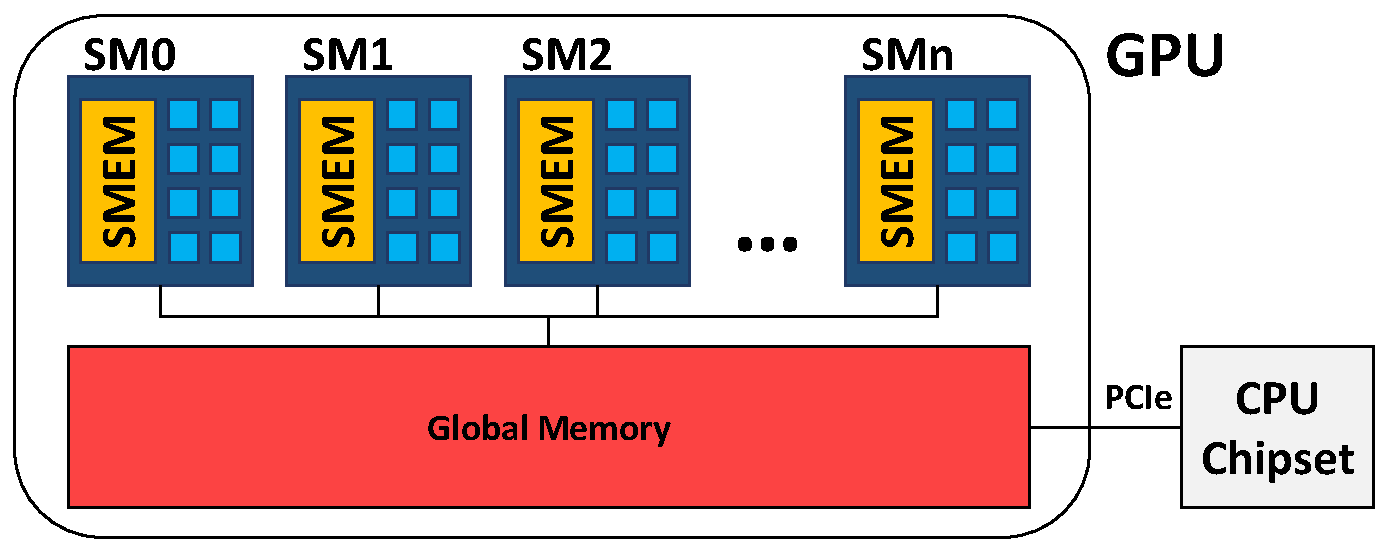
\includegraphics[width=\textwidth]{images/gpuarchitecture.pdf}%memory-hierarchy.png
\caption{The memory hierarchy of Nvidia GPUs (simplified view, adapted from \cite{nvidia_cuda_2012}}
\label{fig:memoryhier}
\end{figure}

\ifdebug
\begin{itemize}
\item History
\item Memory model (important since "computation is for free"
\item Libraries (cuRAND, Thrust) (It's hard to get it right $\rightarrow$ use them)
\item Cross-platform GPGPU library that combined SIMD and multi-threading. Branches should be avoided. 
\item Developer implements kernel, a C function that is loaded from the host (the CPU) to the device (the GPU). It is replicated in many copies named threads. Threads can be organized in three-dimensional structures named blocks which, in turn are part of a grid. 
\item Whenever the host calls a kernel, the device automatically creates the corresponding grid and schedules each block on one streaming multiprocessor (SM) available on the GPU. 
\item Hardware constraints: Block size, registers, blocks per SM, shared memory, ...
\item Warp: 32 threads
\item Memory: shard, global, registers, ... Go beyond the scope of this thesis. 
\item Goal: Have enough memory transactions in flight to hide latency
\end{itemize}
\fi

\subsection{Implementation}
\label{ch:gpuimplementation}
In this chapter the tau-leaping simulator developed in the context of the thesis will be presented. At first, general execution steps of the program and implementation details are discussed. Afterwards, some of the main ideas that were incorporated into the application are explained in more detail. This chapter is solely explanatory in character, the results of numerical validation and performance evaluation experiments will be presented in chapter~4. 

Algorithm \ref{alg:pseudogpu} gives a pseudocode description of the GPU implementation of the tau-leaping algorithm developed for this thesis. Considering the Gray-Scott model as the primary example of this work, the description below represents the special case for $N = 2$ species. It can, however, easily be generalized. In the following the central parts of the implementation are presented in more detail. 

\begin{enumerate}
\item \textbf{Initialization:} During the initialization stage of the application memory for the simulation state is reserved. On the device, two arrays of datatype Integer (int) are reserved to store the number of particles of each species. In the concrete example the arrays are named \texttt{d\_X1a}, \texttt{d\_X1b}, \texttt{d\_X2a} and \texttt{d\_X2b} where \texttt{X1} and \texttt{X2} represent species U and V, respectively. The size of the arrays depends on the number of compartments the system consists of. For example, if the cubic domain of a system is divided into 128x128x128 subvolumes (and assuming \texttt{sizeof(int) = 4}), one array occupies 8 MB of global memory space. To allow parallel execution of the algorithm, two fields for every species are needed to store the previous and the modified state of the system. Furthermore, if negative populations are observed after a leaping step, the old state can easily be reverted. 

Furthermore, two additional arrays have to be allocated on the GPU: \texttt{d\_states} and \texttt{d\_tau\_per\_cell}. The former is used to store the state structures of the pseudo random generators used in the simulation. For the choice presented in the next section, the maximum size is 48 Byte times the number of compartments. The latter is an integral part of the procedure to calculate the leap-length $\tau$ according to equation~\eqref{eq:tau}. Its size depends on the number of CUDA-blocks spawned on the device during the simulation, it contains floating point numbers, i.e.\ \texttt{float} in the given example. The array contains the minimum value derived from the state of the individual compartments of a block. To determine the value of $\tau$ that is used for the next simulation step, the minimum of the values in the array has to be found. A more detailed explanation of the procedure is given in part \ref{enum:4} of this enumeration. 

After being allocated, the values of the device arrays are set by invocating an initialization kernel. It creates and correctly seeds the PRNG states. In addition, the prescribed initial conditions are evaluated and stored in the species state arrays. 

In order to write the state of the simulation to a file, it is necessary to copy the data from the GPU's global memory to the host main memory. This is the reason why on the host an array of the same size has to be allocated for each species of interest. The prefixes '\texttt{d\_}' and '\texttt{h\_}' are used by convention to distinguish between host and device arrays. To achieve best data transfer performance, it is important to use so-called pinned memory, i.e.\ host-side memory that cannot be swapped out to disk by the operating system so that it is instantly available for Direct Memory Access (DMA) copying. Pinned memory can be allocated by library functions that are part of the CUDA framework. 
\label{enum:init}

\item \textbf{CPU-GPU-interaction:} One of the traditional shortcomings of CUDA and GPU computing in general is the fact that complex control flows cannot be handled on the device. Furthermore, kernels can only be launched by the host, not from within GPU code. For the presented tau-leaping implementation this means that the main simulation loop (\texttt{while t < t\textsubscript{end}}) is run on the CPU. Even though all important computations are done in GPU memory, some values such as the proposed tau value or the information if negative populations have been detected must be transferred to the host. If the whole simulation procedure was be manged by the device itself, a lot of time-consuming communication could be avoided. In practice however, implementing the whole algorithm in one complex kernel would neither help achieve high-performance (due to unavoidable branching) nor would it be possible at all (lack of global synchronization). 

On modern Nvidia devices (compute capability $\geq$ 3.0) a feature called Dynamic Parallelism enable kernel invocation within GPU code. Since the tau-leaping simulator presented in this thesis was developed for previous generation hardware (i.e.\ compute capability 2.0), the feature could not be exploited. However, it seems to be promising and should be considered for future work (see \ref{ch:outlook}). 

\item \textbf{Random number generation:} To imitate the stochastic behaviour of the simulated system, any SSA is highly dependent on availability, quality and performance of random number generators. In practice random number generation is usually the computationally most demanding part of the algorithm. The cuRAND library by Nvidia offers several different pseudo-random number generator implementations that support various statistical distributions. The manufacturer claims that the library can outperform CPU-based solutions on current-generation hardware by a factor of almost two orders of magnitude. In the tau-leaping simulation a great number of Poisson-distributed random numbers with varying mean are needed, a functionality that cuRAND offers since version~5.0. XORWOW \cite{saito_variants_2010} is used as the underlying PRNG since it is a good compromise between performance (i.e.\ gigasamples/second), state size and statistical correctness. 

\item \textbf{Thrust library:} In CUDA, "common and important data parallel primitives [are] easy to implement [, but it is] harder to get it right" (Harris, 2007). To increase developer efficiency as well as application performance, several CUDA libraries have been introduced to provide easy access to highly-optimized algorithms and subroutines. The Thrust library of parallel algorithms \cite{hoberock_thrust:_2010}, for example, is shipped directly with the CUDA toolkit. It closely resembles the C++ Standard Template Library (STL) known to many developers. Its performance in benchmarks as well as in real-world application is considered to be out of reach for the average researcher who uses CUDA for simulations. In the tau-leaping implementation presented in this thesis two operations provided by thrust are of great importance: parallel minimum reduction and predicate-based logical reduction. The former is used to find the minimum value of $\tau$ proposed by the compartments stored in the \texttt{d\_tau\_per\_cell} array (see \ref{enum:init}). The latter, more precisely the function \texttt{thrust::any\_of} together with the unary predicate \texttt{is\_negative} is applied to the modified state arrays of both species X1 and X2. It is used to determine if the proposed step has produced negative molecule populations and, if that is the case, it has to be rejected. 

\item \textbf{Tau Selection Procedure:} \label{enum:4}
A good example of how library functions and custom CUDA-kernels by the developer can go hand in hand is the implementation of the tau-selection procedure according to equation \ref{eq:tau}. In a first step, the values for $g_i$ and $x_i$ can be determined by the individual thread. Due to the spatial dependency in the simulated system introduced by diffusion, to calculate the mean $\mu_i$ and the variance $\sigma_i^2$ it is necessary that the molecule population counts of the neighbouring compartments are known. To reduce the number of expensive accesses to global memory, shared memory is used to exploit the principle of data locality within the three-dimensional blocks. Further on, after every thread has calculated its individual tau value, the block-wise minimum of the proposed values is found via reduction in shared memory. Once the kernel has finished execution, the final value for $\tau$ is determined by the high-performance reduction routines provided by Thrust. 

\item \textbf{Reaction kernel:} Implementing the in-compartment reactions \eqref{eq:r1} - \eqref{eq:r4} is straightforward. In the common framework to classify parallel functions \texttt{kernel\_reactions} implements a map operation. In the concrete example this means that every thread reads two values from distinct positions in two arrays (i.e.\ the molecular population counts of its compartment) and writes two values to distinct positions in two other arrays (i.e.\ the molecular counts after the reactions have fired). The operation does not require any synchronization, nor can GPU resources apart from global memory be used to speed up the computation. 

\item \textbf{Diffusion kernel:} Implementing the diffusion kernel and achieving good performance, on the other hand, is much more difficult. Several different approaches can be taken and features of the underlying hardware can be used to accelerate the computation. In the following the main ideas of three different diffusion kernels will be presented. The results of performance analysis will be presented together with other optimization techniques in chapter \ref{ch:gpuopt}. 
\begin{enumerate}
\item \textbf{diffusion\_naive:} This first approach does not make use of shared memory and relies heavily on atomic operations (also called atomics). At first, every thread loads the population counts of the own and neighbouring compartments from global memory. These accesses are not only redundant (every value is needed by 7 threads in 3D), but also strided due to the layout of the compartments in memory (x is the fastest direction, z the slowest). If a thread with three-dimensional index $(i,j,k)$ needs to access a value at $(i+1,j,k)$ (i.e.\ the neighboring compartment in positive x-direction), it can be found right next to its own value. If, however, $(i,j,k+1)$ is accessed, $L^2$ values are in between. Since memory is always accessed in lines, this will definitely affect performance. Considering, for example, Double Data Rate (DDR) memory and a 384 bit wide memory bus, with every memory transaction 24 integer values can be accessed. If just one value is actually needed, only a small fraction of the theoretical peak bandwidth is used. 
When a thread has fetched all the values it needs, it uses Poisson-distributed random variables to determine how many molecules leave the compartment through the six (2D: 4) faces. These numbers then need to be added to or subtracted from the respective values in the state arrays. These accesses are again strided and atomic operations need to be used to avoid data races. Every position in the array is written to seven times and if two or more threads try to modify the value at the same time, incorrect result may be obtained. 

Even though no performance data will be given in this chapter, it is obvious that this first naive approach leaves a lot of space for improvements. Due to the simplicity of the actual code it is suitable to show correctnes of the algorithm and it can act as a reference for more sophisticated approaches. 
\item \textbf{diffusion\_shared} One obvious way to improve the naive approach is to make use of shared memory. If all population counts belonging to threads in a three-dimensional cubic block are stored locally at the SM, almost 6 out of 7 global memory transactions can be saved. Furthermore, the relative performance of strided access patterns and atomic operations in shared memory is overproportionally good compared to global memory. To ensure that in a first step all necessary values have been loaded, all threads in a block have to be synchronized by a barrier. Afterwards, diffusion can be simulated the same way it was described above, this time in fast shared memory instead of slow global memory. When all those operations have finished, the resulting delta-values (i.e.\ the difference between old and new state) are added to the global memory arrays. Compartments at the outer shell of one block are accessed by threads from at least one neighbour (up to three at the corners) so that atomics are needed to ensure correct results. 

An additional challenge that arises from this approach is question of how to handle accesses to neighbouring compartments that are not part of the same block. The simplest idea to handle 'out-of-block reads' is to just fall back to global memory. Since these values are only needed by one thread, there is no use in storing them in shared memory. For 'out-of-block writes' so-called overflow buffers can be introduced. Whenever a delta-value is supposed to be added to an 'out-of-block' compartment, it is stored in this temporary field. After all threads of the block have finished their computation of diffusion, the overflow buffers are added to global memory together with the regular delta values. 
% improvement: memory access when writing them back
\item \textbf{diffusion\_four}
The main idea of the third approach presented is to avoid atomic operations in global memory altogether. If the pattern of active blocks resembles that of a three-dimensional chessboard, the overflow buffers are written to positions in the state arrays that are not owned by an active thread. It is termed \texttt{diffusion\_four} due to the four distinct kernel launches that are needed for the approach. The pattern of active blocks is illustrated in figure \ref{fig:four}. Apart from a more complicated index calculation section in the beginning, the kernels work exactly the same like the previously presented approach. Avoiding atomic operations comes at the coast of the overhead introduced by three additional kernel launches. 
\end{enumerate}

\begin{figure}
\centering
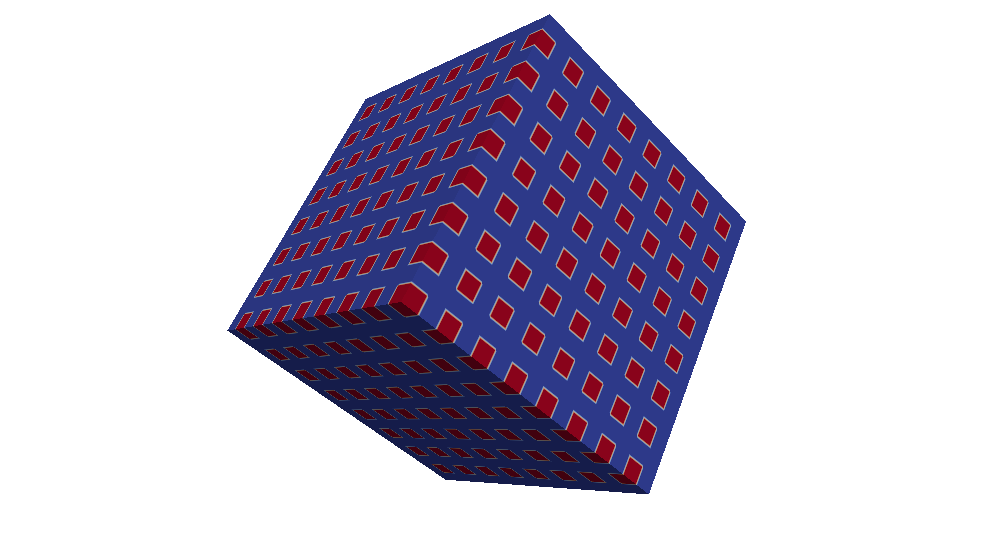
\includegraphics[width=\textwidth]{images/four.png}
\caption{Illustration of the access pattern of \texttt{kernel\_four}. Red blocks are active. }
\label{fig:four}
\end{figure}

It shall be noted that in practice, since all the data that is needed for \texttt{kernel\_reactions} is available within the diffusion kernel, the two are combined to reduce the number of kernel launches and global memory transactions. 
\item \textbf{Output file:} In order to visualize the temporal evolution of the system over time, it is necessary to save the state of the system to the hard drive disk (HDD) in user-defined intervals. For best performance the arrays are written to files in binary, i.e.\ the sequence of bits in the files and in memory is equal. Whenever the control loop on the host enters the output section, data has to be copied from GPU to CPU memory. Since kernel launches in CUDA are asynchronous and input/output operations are managed by the operating system in the background, the application can continue regular execution even before the file has been stored on the comparably slow HDD. Apart from performance considerations one of the main advantages of the binary file format (.bin, .raw) is that it can be read by almost all programs one may use for post-processing. If that is not the case, data can easily be converted with tools such as MATLAB. On the other hand, it shall be noted that binary files are not necessarily interoperable (e.g. depending on system architecture, operating system and compiler different result may be produced), they are not readable for humans and a lot of implicit information such as data type, endianness, system dimension and coordinate axis ordering has to be provided to be able to work with the file. 
\end{enumerate}

%\begin{mdframed}
\begin{algorithm}[H]
\DontPrintSemicolon
%\KwIn{Initial state $\vec{x}_0$, propensity functions $\alpha_j$, time $t_{end}$}
%\KwOut{State $\vec{x}(t)$ for $t \in \lbrack t,t_{end}\rbrack$ (TODO)}
\textbf{Initialization:} \\
Allocate state arrays $\mathtt{d\_X1a}$, $\mathtt{d\_X1b}$, $\mathtt{d\_X2a}$ and $\mathtt{d\_X2b}$ on the device. \\
Allocate random generator state array $\mathtt{d\_states}$ on the device. \\
Allocate local tau array $\mathtt{d\_tau\_per\_cell}$ on the device. \\
Allocate state arrays $\mathtt{d\_X1}$ and $\mathtt{d\_X2}$ on the host. \\
Execute $\mathtt{kernel\_init\_device(d\_X1a,\ldots,d\_X2b,d\_states)}$. \\
Write initial state to file.\;
\textbf{Simulation loop:}\\
Set pointer $\mathtt{d\_X1\_old} \rightarrow \mathtt{d\_X1a}$. \\
Set pointer $\mathtt{d\_X1\_new} \rightarrow \mathtt{d\_X1b}$.  \\
\ldots\footnote{Analogous for $\mathtt{d\_X2\_old}$ and $\mathtt{d\_X2\_new}$.}\\
\While{$\mathtt{t} < \mathtt{t_{end}}$}{
Execute $\mathtt{kernel\_tau\_local(d\_X1\_old,d\_X2\_old,d\_tau\_per\_cell)}$. \\
Set $\mathtt{tau} = \mathtt{thrust::reduce(d\_tau\_per\_cell,thrust::minimum)}$. \;
\While{$\mathtt{true}$}{
Execute \texttt{kernel\_reactions(d\_X1\_prev,\ldots,tau,d\_states)}. \;
Execute \texttt{kernel\_diffusion(d\_X1\_prev,\ldots,tau,d\_states)}. \;
\eIf{$\mathtt{thrust::any\_of(d\_Xi\_new,is\_negative())}$\footnote{For any of the two arrays $\mathtt{d\_X1\_new}$ and $\mathtt{d\_X2\_new}$, i.e.\ $\mathtt{i} = 1,2$.}}{
$\mathtt{tau} = \mathtt{tau / 2}$\;}{
\texttt{break} \;
}
} %end while true
\If{$\mathtt{t} \geq \mathtt{write\_counter} * \mathtt{write\_every}$ }{Write current state to file.}
Swap $\mathtt{d\_X1\_old}$ and $\mathtt{d\_X1\_old}$. \\
Swap $\mathtt{d\_X2\_old}$ and $\mathtt{d\_X2\_old}$. \;
} % end simulation loop
\textbf{Finalization:} \\
Write final state to file. \\
Deallocate arrays and reset device. \;
\caption{Overview for GPU implementation !!!}
\label{alg:pseudogpu}
\end{algorithm}
%\end{mdframed}

\ifdebug
\begin{itemize}
\item Memory limitation: Large systems may exceed on-board capacity of a single GPU $\rightarrow$ spatial decomposition, communication, load balancing, complicated (cite Hallock)
\item The application was compiled with ... It depends on CUDA 6.0 (released...).
\item Thesis comes with code. Can be used..., warranty, ...
\end{itemize}
\fi